\NeedsTeXFormat{LaTeX2e}[1996/06/01]
 \documentclass{cambridge7A}
 \usepackage{natbib}
 \usepackage[figuresright]{rotating}
 \usepackage{floatpag}
 \rotfloatpagestyle{empty}
 \usepackage{mathrsfs}
 \usepackage{xspace}
 \usepackage{amsthm,amsmath}
 \usepackage{graphicx} 
 \usepackage{mathtools}
 \usepackage{txfonts}
 \usepackage{multind}\ProvidesPackage{multind}
 \usepackage{hyperref}
 \usepackage{color}
 \usepackage[lastexercise,answerdelayed]{exercise}
 \usepackage[all]{xy}
 \usepackage{alltt}
 \usepackage[shortlabels]{enumitem}
 \usepackage{mik-makro}
    \usepackage{tikz-cd}
 \makeindex{authors}
 \makeindex{subject} 
 \makeglossary
 \theoremstyle{plain}% default
 \newtheorem{theorem}{Theorem}[chapter]
 \newtheorem{lemma}[theorem]{Lemma}
 \newtheorem{claim}[theorem]{Claim} 
 \newtheorem{proposition}[theorem]{Proposition}
 \newtheorem{corollary}[theorem]{Corollary}
 \newtheorem{conjecture}[theorem]{Conjecture}
 \newtheorem*{theorem*}{Theorem}
 \newtheorem*{lemma*}{Lemma} 
 \newtheorem*{proposition*}{Proposition}
 \newtheorem*{corollary*}{Corollary}
 \newtheorem*{conjecture*}{Conjecture}
 \theoremstyle{definition}
 \newtheorem{definition}[theorem]{Definition}
%  \newtheorem{myexample}[theorem]{myexample}
 \newtheorem{prob}[theorem]{Problem}
 \newtheorem{remark}[theorem]{Remark}
 \newtheorem{notation}[theorem]{Notation}
 \newtheorem{exer}[theorem]{Exercise}
 \newtheorem*{definition*}{Definition}
 \newtheorem*{example*}{myexample}
 \newtheorem*{prob*}{Problem}
 \newtheorem*{remark*}{Remark}
 \newtheorem*{notation*}{Notation}
 \newtheorem*{exer*}{Exercise}
 \setcounter{tocdepth}{2}
 \newcommand\cambridge{cambridge7A}
 \def\makeRRlabeldot#1{\hss\llap{#1}}
 \renewcommand\theenumii{{\rm (\roman{enumii})}}
 \renewcommand\theenumi{{\rm (\arabic{enumi})}}
 \renewcommand\theenumiii{{\rm (\alph{enumiii})}}
 \renewcommand\theenumiv{{\rm (\Alph{enumiv})}}


 \newcommand{\mikexercise}[2]{
\begin{mexercise} 
	#1 
	% #2
\end{mexercise}

\smallskip
\noindent{\bf Solution.} #2

\vfill
\pagebreak
    }



 \begin{document}
 \newcommand{\decisionproblem}[2]
{
	\begin{itemize}
		\item {\bf Input.} #1
		\item {\bf Output.} #2
	\end{itemize}
}

\newcommand{\freevar}[1]{\mathrm{var}(#1)}

\newcommand{\fdp}{\textsc{fdp}\xspace}

\newcommand{\pspace}{{\sc{PSpace}\xspace}}
\newcommand{\indvec}[1]{\atoms^{\langle #1 \rangle}}
 \newcommand{\dimension}[1]{\mathrm{dim}(#1)}
\newcommand{\leastsup}[1]{\mathrm{sup}(#1)}

\newcommand{\syntdim}[1]{\mathrm{dim}(#1)}
\newcommand{\syntsize}[1]{|#1|}
\newcommand{\semdim}[1]{\mathrm{\red{dim}}(#1)}
\newcommand{\semsize}[1]{\red|#1\red|}

\newcommand{\orbitsize}[2]{|#1|_{#2}}
%\newcommand{\saut}[1]{\mathrm{G}_{#1}}
%\newcommand{\aut}{\mathrm{G}}
%\newcommand{\secfm}{\bfseries{\scshape{fm\ }}}
%\newcommand{\fm}{\textsc{fm}\ }
%\newcommand{\tneq}{\(\neq\)}
\newcommand{\tleq}{\(\leq\)}
% \newcommand{\tin}{\(\in\)}
% \newcommand{\tnotin}{\(\notin\)}
% \newcommand{\tcup}{\(\cup\)}
% \newcommand{\temptyset}{\(\emptyset\)}
% \newcommand{\tcap}{\(\cap\)}
% \newcommand{\ttimes}{\(\times\)}

\newcommand{\approxi}[2]{#1^{(#2)}}

\newcommand{\cellc}[2]{\mathsf{cell}_{#1}(#2)}
\newcommand{\tatoms}{\(\ \!\!\!\!\atoms\)}

% \newcommand{\booltrue}{\ensuremath{\mathtt{true}}}
% \newcommand{\boolfalse}{\ensuremath{\mathtt{false}}}
\newcommand{\tset}[1]{\{#1\}}

\newcommand{\settype}{\mathtt{set}}
\newcommand{\atomtype}{\mathtt{atom}}

\newcommand{\red}[1]{{\color{red}#1}}
\newcommand{\blue}[1]{{\color{blue}#1}}

\newcommand{\exercisepart}{

\bigskip

{\noindent \large \bf Exercises}


}
\newcommand{\setexpr}[3]{\set{#1\ |\ \text{ for }#2 \in \atoms \text{ such that }#3}}
\newcommand{\setexprtup}[4]{\set{#1\ |\ \text{ for }#2 \in \atoms^{#3} \text{ such that }#4}}
\newcommand{\setexprtrue}[2]{\set{#1\ |\ \text{ for }#2 \in \atoms}}
\newcommand{\setexprtuptrue}[3]{\set{#1\ |\ \text{ for }#2 \in \atoms^{#3}}}

\newcommand{\symbolpushbis}[2]{\symbolpush{#1 \ : \ #2}}
\newcommand{\symbolpush}[1]{\underline{#1}}

\newcommand{\aequiv}[1]{\stackrel{#1}\sim}
\newcommand{\locations}{\mathsf{Loc}}

\newcommand{\bibnotes}[1]{
\bigskip
{\footnotesize
\noindent {\bf Bibliographic notes for Section~\arabic{section}. }
#1}
}

% these two macros are for delayed exercises, I don't use them now
% \renewcommand{\ExerciseHeader}{\noindent \textbf{\ExerciseName~\ExerciseHeaderNB\ExerciseHeaderTitle
% \ExerciseHeaderOrigin. }}
% \renewcommand{\AnswerHeader}{\noindent {\textbf{Solution to \ExerciseName\ \ExerciseHeaderNB.\\}}}

\newcounter{exercisecounter}
\newenvironment{mexercise}{
\refstepcounter{exercisecounter}

\smallskip\noindent{\textbf{{Exercise \arabic{exercisecounter}. }}}}{
}






\newcommand{\pv}[1]{{\mathtt{#1}}}

% the original picture files, from illustrator
\newcommand{\mypic}[1]{
\begin{center}
	\includegraphics[page=#1,scale=0.5]{pictures/from-ai}
\end{center}
}

% for pictures with figma
\newcommand{\mypicb}[1]{
\begin{center}
	\includegraphics[page=#1,scale=0.22]{pictures/atom-book}
\end{center}
}

%\newcommand{\notin}{\not \in}

\newcommand{\sets}{\mathsf{set}}
\newcommand{\setbuil}{\mathsf{setbuil}}
\newcommand{\defset}{\mathsf{hdef}}
\newcommand{\hofset}{\mathsf{hof}}

\newcommand{\setbuild}[2]{\set{\ #1 \ | 
\begin{tabular}{l}
	#2
\end{tabular}}}

% the tabular in the above macro can make it too wide, hence this one
\newcommand{\setbuildoneline}[2]{\set{\ #1 \ | 
\text{ #2}\ }}

\newcommand{\myunderbrace}[2]{\underbrace{#1}_{\mathclap{\text{\scriptsize 
\begin{tabular}{c}
	#2
\end{tabular} }}}}
\newcommand{\myoverbrace}[2]{\overbrace{#1}^{\mathclap{\text{\scriptsize 
\begin{tabular}{c}
	#2
\end{tabular} }}}}

\newcommand{\Bool}{2}
\newcommand{\eve}{\text{Eve}}
\newcommand{\adam}{\text{Adam}}
\newcommand{\john}{\text{John}}
\newcommand{\tom}{\text{Tom}}
\newcommand{\jim}{\text{Jim}}
\newcommand{\mary}{\text{Mary}}

\newcommand{\deflift}{{\mathsf{def}}}
\newcommand{\tti}{{\mathtt I}}
\newcommand{\ttj}{{\mathtt J}}
\newcommand{\qatom}{(\mathbb Q, <)}
\newcommand{\sem}[1]{[\![#1]\!]}
\newcommand{\fraisse}{Fra\"iss\'e } 

\newcommand{\saut}[1]{\mathrm{G}_{#1}}
\newcommand{\aut}{\mathrm{G}}
\newcommand{\secfm}{\bfseries{\scshape{fm\ }}}
%\newcommand{\fm}{\textsc{fm}\ }
\newcommand{\tneq}{\(\neq\)}
\newcommand{\tin}{\(\in\)}
\newcommand{\tnotin}{\(\notin\)}
\newcommand{\tcup}{\(\cup\)}
\newcommand{\temptyset}{\(\emptyset\)}
\newcommand{\tcap}{\(\cap\)}
\newcommand{\ttimes}{\(\times\)}

\newcommand{\structclass}{\mathscr A}
\newcommand{\structclassb}{\mathscr B}
\newcommand{\structclassh}{\mathscr H}
\newcommand{\structa}{\mathbb A}
\newcommand{\structb}{\mathbb B}
\newcommand{\structc}{\mathbb C}
\newcommand{\structh}{\mathbb H}

\newcommand{\atoms}{\mathbb A}
\newcommand{\field}{\mathbb F}
\newcommand{\universe}[1]{\mathrm{universe(#1)}}
\newcommand{\Fff}{\mathscr F}
\newcommand{\limmodel}{\underline \structa}
\newcommand{\arity}{\mathrm{arity}}
\newcommand{\lincomb}{\mathrm{Lin}}
\newcommand{\length}{\mathrm{len}}

% various kinds of function spaces
\newcommand{\lineqfun}[2]{ #1 \underset{\text{lineq}}{\longrightarrow} #2}
\newcommand{\linfsfun}[2]{ #1 \underset{\text{linfs}}{\longrightarrow} #2}
\newcommand{\eqfun}[2]{ #1 \underset{\text{eq}}{\longrightarrow} #2}
\newcommand{\fsfun}[2]{ #1 \underset{\text{fs}}{\longrightarrow} #2}

\newcommand{\generate}[1]{\langle #1 \rangle}

\newcommand{\atoma}{{a}}
\newcommand{\atomb}{{b}}
\newcommand{\atomc}{{c}}
\newcommand{\atomd}{{d}}

\newcommand{\atomq}{{q}}
\newcommand{\atomzero}{{\underline 0}}
\newcommand{\atomone}{{\underline 1}}
\newcommand{\atomtwo}{{\underline 2}}
\newcommand{\atomthree}{{\underline 3}}

 
\newcommand{\atomseta}{{A}}
\newcommand{\atomsetb}{{B}}
\newcommand{\atomsetc}{{C}}
\newcommand{\atomsets}{{S}}
\newcommand{\atomsett}{{T}}

\newcommand{\Qfin}{Q_{\mathrm{fin}}}
\newcommand{\Afin}{A_{\mathrm{fin}}}

\newcommand{\bind}{\nabla}
\newcommand{\powerset}{{\mathsf P}}
\newcommand{\pfin}{{\mathsf P}_{\text{fin}}}
\newcommand{\decproblem}[3]
{\begin{center}
\fbox{
\begin{tabular}{rl}
\textsc{Problem}: & #1 \\
\textsc{Input}: & #2\\
\textsc{Output}: & #3
\end{tabular}
}
\end{center}}

\newcounter{openquestioncounter}
\newenvironment{openquestion}{
\medskip

\refstepcounter{openquestioncounter}
\smallskip\noindent{\textbf{{Open question \arabic{openquestioncounter}. }}}}{\hfill $\Box$
\medskip 
}







\newcommand{\eqdef}{\stackrel {\mathrm{def}} = }

\newcommand{\Ii}{\mathcal I} 

% chapter 1: pof sets
\mikexercise{\label{pof-one-way-permutation} In the definition of an equivariant subset from Definition~\ref{def:equivariant-pof}, we have an equivalence $\Leftrightarrow$, and we quantify over atom permutations, which can be briefly written as
\begin{center}
    \begin{tabular}{lllll}
        0.  & 
        $\bar a \in X$ & $\Leftrightarrow$ & $\pi(\bar a) \in X$ 
        & for all permutations $\pi : \atoms \to \atoms$.
    \end{tabular}
\end{center}
Instead of a two-way implication, we can have a one-way implication in either of the two directions, and we can quantify over functions that are not necessarily permutations, as in the following variants:
\begin{center}
    \begin{tabular}{lllll}
        1.  & 
        $\bar a \in X$ & $\Rightarrow$ & $\pi(\bar a) \in X$ 
        & for all permutations $\pi : \atoms \to \atoms$\\
        2.  & 
        $\bar a \in X$ & $\Leftarrow$ & $\pi(\bar a) \in X$ 
        & for all permutations $\pi : \atoms \to \atoms$\\
        3.  & 
        $\bar a \in X$ & $\Leftrightarrow$ & $\pi(\bar a) \in X$ 
        & for all functions $\pi : \atoms \to \atoms$\\
        4.  & 
        $\bar a \in X$ & $\Rightarrow$ & $\pi(\bar a) \in X$ 
        & for all functions $\pi : \atoms \to \atoms$\\
        5.  & 
        $\bar a \in X$ & $\Leftarrow$ & $\pi(\bar a) \in X$ 
        & for all functions $\pi : \atoms \to \atoms$
    \end{tabular}
\end{center}
Which variants are equivalent to the original definition, as in variant 0?}{ Variants 0,1,2 are equivalent to each other, and stronger than all  the other variants. Variant 3 is the weakest one, weaker than all the others. Finally, variants 4 and 5 are incomparable to each other, and set between 0=1=2 and 3. Here is a more detailed explanation:
    \begin{enumerate}
        \item     This variant, which uses an implication $\Rightarrow$ and atom permutations is equivalent to the original definition. This is because  permutations have inverses. The right-to-left implication 
        \begin{align*}
            (a_1,\ldots,a_d) \in X 
            \quad \Leftarrow \quad
            (\pi(a_1),\ldots,\pi(a_1)) \in X
            \end{align*}
        follows from  the left-to-right implication  (we use different variable names for clarity)
        \begin{align*}
            (b_1,\ldots,b_d) \in X 
            \quad \Rightarrow \quad
            (\sigma(b_1),\ldots,\sigma(b_1)) \in X
            \end{align*}
        in the special case of  $\sigma = \pi^{-1}$ and $b_i = \pi(a_i)$. 
        \item Also, equivalent to the original definition, for the same reasons as above. 
        \item If $X$ is of the form $\atoms^d$, then this variant only enables the full or empty sets. In particular, it is not equivalent to the original definition, since that definition enables other sets than full or empty.  Indeed, using the implication $\Rightarrow$ and the function that maps all atoms to the same atom $a$,   we conclude that if $X$ contains at least one tuple, then it must contain the tuple 
            \begin{align*}
            (a,a,\ldots,a)
            \end{align*}
        that uses  atom $a$ on all coordinates.  Using the same function and the converse implication $\Leftarrow$, we conclude that the set must contain all tuples in $\atoms^d$. 
        \item This variant is weaker than 0=1=2, but it is stronger than 3. Clearly, we have the implications 
            \begin{align*}
            3 \quad \Rightarrow \quad 4 \quad \Rightarrow \quad 0=1=2.
            \end{align*}
        It remains to show that the implications are strict: 
            \begin{enumerate}
                \item the diagonal $\setbuild{(a,a)}{$a \in \atoms$} \subseteq \atoms^2$ is consistent with this variant, but not with variant 3;
                \item the complement of the diagonal is not consistent with this variant, but is consistent with variants 0=1=2.
            \end{enumerate}
        \item The same discussion as in the previous point applies here.
    \end{enumerate}

}



\mikexercise{\label{pof-cant-create-atom} Show that there is no equivariant function of type $\atoms^0 \to \atoms$.}{
    If the graph of this function would contain 
    \begin{align*}
    () \mapsto a
    \end{align*}
    then for every atom permutation $\pi$ it  would also need to contain 
    \begin{align*}
    \pi(()) \mapsto \pi(a),
    \end{align*}
    which is the same as 
    \begin{align*}
    () \mapsto \pi(a).
    \end{align*}
    Therefore,  it would not be a function.
}

\mikexercise{\label{pof-number-of-subsets} Show that the number of equivariant subsets of  $\atoms^{d}$ is doubly exponential in $d$.  
}{
    Equivariant subsets are the same thing as unions of orbits. We know that the number of orbits is exponential, so the number of their unions is doubly exponential.
}

\mikexercise{\label{pof-transitive-relation-closure}Consider a pof set $X$ and an equivariant binary relation $R \subseteq X \times X$. Show that the transitive closure of $R$ is also equivariant.}{
    A pair $(x,y)$ belongs to the transitive closure if and only if there is a sequence 
    \begin{align*}
    x = x_1,\ldots,x_n = y
    \end{align*}
    such that $R(x_i,x_{i+1})$ holds for  all $i \in \set{1,\ldots,n-1}$. To such a sequence we can apply a permutation $\pi$ to get a new sequence 
    \begin{align*}
        \pi(x) = \pi(x_1),\ldots,\pi(x_n) = \pi(y),
        \end{align*}
    which witnesses that $(\pi(x), \pi(y))$ is in the transitive closure. Therefore, the transitive closure is closed under applying atom permutations, i.e.~it is equivariant.
}



\mikexercise{
\label{ex:equal-subsets}    
Consider the following problem: given two subsets of a pof set decide if they are equal. Show that this problem is: (a) in deterministic logarithmic space under the generating set representation; and (b) complete for coNP under the formula representation.}{
    This problem is complete for coNP. 
}



\mikexercise{To specify a subset of $X \subseteq \atoms^d$, we can also use a formula with quantifiers (which range over atoms). 
 Show that for every such formula, there is an equivalent formula that is quantifier-free. For example, the formula 
 \begin{align*}
 \varphi(x_1,x_2) = \exists y \ (x_1 \neq y) \land (x_2 \neq y),
 \end{align*}
 is equivalent to ``true''.
}{
    Even with quantifiers, formulas can only define equivariant subsets. This is shown by induction on formula size. Equivariant subsets, in turn, can be defined in a quantifier-free way.
}

% chapter 2: pof automata
\mikexercise{\label{pof-undirected-reachability} Show that the reachability problem remains \textsc{PSpace}-complete when we restrict it to symmetric graphs, i.e.~graphs where the edge relation is symmetric\footnote{Note that in the case of finite graphs, the complexity drops from NL to L when restricting to symmetric graphs, as shown  in~\cite{reingold2008undirected}.}. }{}

\mikexercise{\label{pof-spanning-tree} Consider an undirected pof graph, i.e.~a graph where the edge relation is symmetric.   Does it necessarily have a spanning tree that is equivariant?}{
    No. Consider the clique on the vertex set $\atoms$. If a hypothetical equivariant spanning tree would contain an edge $ab$ for some atoms $a \neq b$,  it would need to contain every such edge.
}

\mikexercise{\label{pof-graph-isomorphism}Consider two undirected pof graphs, which are isomorphic. Is there necessarily an isomorphism that is equivariant? }{ No. Consider the cliques on $\atoms$ and $\atoms^2$. A hypothetical isomorphism would need to be a bijection between the two sets, and no such bijection exists. This is a because there is only one  equivariant function of type $\atoms \to \atoms^2$, namely $a \mapsto (a,a)$. }


\mikexercise{\label{pof-graph-diameter}
    Show that given a directed pof graph,  one can compute a number $k \in \set{0,1,\ldots}$ such that for every two vertices $s$ and $t$, if there is a path from $s$ to $t$, then there is a path of length at most $k$. 
}
{
    Define $R_n \subset V \times V$ to be the binary relation which tells us which pairs can be reached by a path of length at most $n$. This relation is defined by the equations 
    \begin{align*}
    R_0 = \set{ (v,v) \mid v \in V} \\
    R_{n+1} = R_n \circ E \cup R_n.
    \end{align*}
    By definition, we have a chain
    \begin{align*}
        R_0 \subset R_1 \subset R_2 \subset \cdots.
    \end{align*}
    Since $R_{n+1}$ is defined based on $R_n$, it follows that if the chain has two consecutive equal elements, then all subsequent elements are equal. Such equal elements must occur, since all relations $R_n$ are equivariant subsets of $V \times V$, and there are finitely many such subsets. Therefore, the chain stabilizes after some finite number of steps, thus giving the bound in the problem. All of this can be computed.
}

\mikexercise{\label{pof-infinite-path-in-graph}
    Consider a directed pof graph. Show that there is an infinite path if and only if there is a cycle.
}
{
    Up to atom permutations, there are finitely many vertices. Therefore, if there is an infinite path, then there is a path $v \to w$ such that $v$ and $w$ are equal up to atom permutations, i.e.~there is some atom permutation $\pi$ such that $w = \pi(v)$. We can choose this permutation so that it moves only finitely many atoms, namely those that appear in $v$. Since reachability is equivariant, we know that there is an infinite path
    \begin{align*}
        \pi^0(v) \to \pi^1(v) \to \pi^2(v) \to \cdots .
    \end{align*} 
    By the assumption that $\pi$ moves finitely many atoms, we know that for some $n$, the permutation $\pi^n$ is the identity, and thus the path returns to the original vertex $v$. 
}

\mikexercise{\label{pof-graph-acyclic-upper-bound}
    Consider a  directed pof graph. Show that if the graph is acyclic, then there is a finite upper bound $k$ on the length of paths.
}{
    If paths had unbounded length, then we could find a path $v \to w$ such that $v$ and $w$ are in the same orbit. Using the same argument as in the previous problem, we could get an infinite path. 
}

\mikexercise{\label{pof-finite-outdegree}Show that the following problem is decidable: given a directed pof graph, decide if it has finite outdegree, i.e.~for every vertex $v$, there are finitely many vertices $w$ with an edge $v \to w$. }
{
We will show that  a pof directed graph has infinite outdegree if and only if 
\begin{itemize}
    \item[(*)] there is some edge $v \to w$ such that some atom from $w$ does not appear in $v$.
\end{itemize} 
This will solve the problem, since (*) is easily seen to be decidable. Let us now prove the equivalence. Clearly if (*) holds, then the outdegree of $v$ is infinite, since the atom that does not appear in $v$ can be chosen in infinitely many possible ways. Conversely, if (*) does not hold, then for every $v$ there are finitely many possible choices for $w$ with $v \to w$, because there are finitely many elements in a pof set that use a give finite set of atoms.
}


\mikexercise{\label{ex:no-infinite-finitely-supported-path} Assume the equality atoms. Show a graph which has an infinite path, but does not have any infinite finitely supported path.}{ The vertices are nonrepeating tuples of atoms, and there is an edge $\bar a \to \bar b$ whenever $\bar a$ is a proper prefix of $\bar b$. This graph clearly contains an infinite path, but every such path uses infinitely many atoms, and is therefore not finitely supported. 
}





\mikexercise{\label{pof-example-dfa-first-last}Find a deterministic pof automaton for the following language:
\begin{eqnarray*}
\setbuild{w \in \atoms^*}{the first and last letters are different}.
\end{eqnarray*}
\vspace{-0.6cm}
}
{
The state space of the automaton is 
    \begin{align*}
    \underbrace{\atoms^0}_{\text{initial}} + \underbrace{\atoms}_{\text{yes}} + \underbrace{\atoms}_{\text{no}}
    \end{align*}
    The unique state in the first component is the  initial state. The states in the second and third components store the first letter, with the second component  corresponding to words in the language, and the third component corresponding to words not in the language. The accepting set consists of the states in the second component $\gamma$. The transition function is:
    \begin{align*}
    \text{initial}()  & \stackrel a \to \text{no}(a) \\
    \text{yes}(a) & \stackrel b \to 
    \begin{cases}
    \text{yes}(a) & \text{if $a = b$} \\
    \text{no}(a) & \text{if $a \neq b$}
    \end{cases} \\
    \text{no}(a) & \stackrel b \to 
    \begin{cases}
    \text{yes}(a) & \text{if $a = b$} \\
    \text{no}(a) & \text{if $a \neq b$}.
    \end{cases} 
    \end{align*}

}

\mikexercise{\label{pof-example-dfa-two-consecutive}Find a deterministic pof automaton for the following language:
\begin{eqnarray*}
    \setbuildoneline{w \in \atoms^*}{no two consecutive letters are the same}. 
\end{eqnarray*}
\vspace{-0.6cm}
}
{
    The state space of the automaton is 
    \begin{align*}
    \underbrace{\atoms^0}_{\text{initial}} + \underbrace{\atoms}_{\text{noninitial}} + \underbrace{\atoms^0}_{\text{error}}.
    \end{align*}
    The unique state in the first is the initial state, and the last component  represents a rejecting sink state. The accepting states are those from the first two  components. The atom in the component $\beta$ stores the most recently seen atom. Here is the transition function: 
    \begin{align*}
    \text{initial}()  & \stackrel a \to \text{non-initial}(a) \\
    \text{non-initial}(a) & \stackrel b \to
    \begin{cases}
        \text{non-initial}(b) & \text{if $a \neq b$} \\
        \text{error}() & \text{if $a = b$}
    \end{cases}\\
    \text{error}() & \stackrel b \to \text{error}().
    \end{align*}
}

\mikexercise{\label{ex:at-least-three-different}Find a deterministic pof automaton for the language 
\begin{eqnarray*}
    \setbuildoneline{w \in \atoms^*}{there are at least three different letters}.
\end{eqnarray*}
\vspace{-0.6cm}
}
{
    The automaton stores the atoms that have been seen so far, up to three atoms; otherwise it uses a rejecting sink state. The state space of the automaton is 
    \begin{align*}
    \underbrace{\atoms^0}_{\text{seen}_0} + \underbrace{\atoms^1}_{\text{seen}_1} + \underbrace{\atoms^2}_{\text{seen}_2} + \underbrace{\atoms^3}_{\text{seen}_3} + \underbrace{\atoms^0}_{\text{error}}.
    \end{align*}
    After reading an input word that has $i \leq 3$ distinct atoms, the state is $\text{seen}_i(a_1,\ldots,a_i)$, where $a_1,\ldots,a_i$ are the atoms seen in the input word in their order of appearance. In particular, the initial state is $\text{seen}_0()$. The last component is a rejecting sink state; all other states are accepting. The transition function is:
    \begin{align*}
    \text{seen}_0()  & \stackrel a \to \text{seen}_1(a) \\
    \text{seen}_1(a) & \stackrel b \to 
    \begin{cases}
    \text{seen}_2(a,b) & \text{if $b \not\in \set a$} \\
    \text{seen}_1(a) & \text{otherwise}
    \end{cases}\\
    \text{seen}_2(a,b) & \stackrel c \to
    \begin{cases}
    \text{seen}_3(a,b,c) & \text{if $c \not\in \set{a,b}$} \\
    \text{seen}_2(a,b) & \text{otherwise}
    \end{cases}\\
    \text{seen}_3(a,b,c) & \stackrel d \to 
    \begin{cases}
    \text{seen}_3(a,b,c) & \text{if $d \not\in \set{a,b,c}$} \\
    \text{error}() & \text{otherwise}
    \end{cases}
\end{align*}
}

\mikexercise{\label{pof-only-letters-used}
    Consider a deterministic pof automaton. Show that after reading an input string $w$, all atoms that appear in the state must also appear in $w$.}
    {This is a corollary of a more general fact: if we have an equivariant function $f : X \to Y$, for two pof sets $X$ and $Y$, then all atoms that appear in $f(x)$ must also appear in $x$. Let us prove this fact. Equivariance means that if $x \mapsto y$ is an input/output pair for the function $f$, then the same is true for $\pi(x) \mapsto \pi(y)$. Suppose now, toward a contradiction, that there would be some input/output pair $x \mapsto y$ such that some atom $a$ appears in $y$ but not in $x$. Choose some atom permutation $\pi$ that moves the atom $a$ to some other atom, but keeps all atoms from $x$ unchanged. Then $\pi(x) \mapsto \pi(y)$ would also need to be an input/output pair, but since $x=\pi(x)$ and $y \neq \pi(y)$, this would mean that $f$ is not a function. } 

    \mikexercise{\label{pof-dfa-finite-alphabet}Show that if the input alphabet is finite (i.e.~a pof set of dimension zero), then  deterministic pof automata recognise exactly the regular languages.}
    {
        By Problem~\ref{pof-only-letters-used}, the reachable states cannot have any atoms. There are finitely many such states in a given pof set, and hence the automaton can be made finite-state.  
    }

    \mikexercise{\label{pof-reach-path-few-atoms}
    Consider a nondeterministic pof automaton, and let $k$ be the maximal number of atoms that  can appear in a single transition. Let $A$ be a finite set of $k$ atoms.
    Show that if the automaton is nonempty, then it accepts some word that uses only atoms from $A$.
}{ 
    We will show that for every path 
    \begin{align*}
    \rho = q_0 \stackrel{a_1} \to q_1 \stackrel{a_2} \to \cdots \stackrel{a_n} \to q_n
    \end{align*}
    of this automaton, there is another run 
    \begin{align*}
        \rho' = q'_0 \stackrel{a'_1} \to q'_1 \stackrel{a'_2} \to \cdots \stackrel{a'_n} \to q'_n
        \end{align*}
    that  uses only atoms from $A$, and such that the starting states $q_0$ and $q'_0$ are in the same orbit, and the last states $q_n$ and $q'_n$ are also in the same orbit. If we apply this to a run that witnesses nonemptiness, we will get the desired result. 
    
    The proof if by induction on the length $n$ of the run. In the induction base of $n=1$, we simply replace each atom from $q_0$ with some distinct atom from $A$, and there are enough such atoms (here, it would be enough that $A$ has as many atoms as the dimension of $Q$). 

    Consider now the induction step, and suppose that we have already defined the new run  for $n-1$, and we want to extend it to $n$. Consider the last transition 
    \begin{align*}
    q_{n-1} \stackrel{a_n} \to q_n
    \end{align*}
    in the original run $\rho$. The number of atoms used by this transition is at most the size of $A$. Therefore,  we replace these atoms with ones from $A$, in a way that maps $q_{n-1}$ to $q'_{n-1}$ from the induction. This proves the induction step. 
}
    


\mikexercise{\label{pof-derivative}
    Define a left derivative of a language $L \subseteq \Sigma^*$ to be a language of the form 
    \begin{align*}
     v^{-1}w \eqdef   \setbuild{ w \in \Sigma^*}{$vw \in L$}
    \end{align*}
    for some word $v \in \Sigma^*$. Are languages recognised by deterministic pof automata closed under left derivatives?
}{
    This is a bit of a silly trick question. The answer is no, because a left derivative will no longer be equivariant, since the atoms used by $v$ might need to be included  as constants into the automaton recognizing $v^{-1}w$, and atom constants are not allowed in our model. If we allowed atom constants, then the answer would be yes.
}

\mikexercise{\label{pof-myhill}
    We say that two states $p$ and $q$ in a deterministic pof automaton are \emph{behaviourally equivalent} if for every input string $w$, the states $pw$ and $qw$ are both accepting or both rejecting. Show that behavioural equivalence is equivariant.
}
{
    Follows directly from the definitions. 
}
\mikexercise{\label{pof-minimal}
    A deterministic pof automaton is called minimal if one cannot find reachable states $p\neq q$ that are behaviourally equivalent.  Show a language that is recognised by some deterministic pof automaton but not by any minimal deterministic pof automaton.
}{
    Consider the language 
    \begin{align*}
    \setbuild{abc \in \atoms^*}{$a,b,c$ are three distinct atoms}.
    \end{align*}
    This language contains only words of length three. Consider some hypothetical deterministic pof automaton. The states after reading words $ab$ and $ba$ are behaviourally equivalent. However, they will not be the same state, since one is obtained from the other by swapping $a$ with $b$, and such a swap must change the state (unless it does not store the atoms $a$ and $b$, which cannot happen in an automaton that recognises the language).
}

\mikexercise{\label{pof-epsilon-nondet}
    Show that the expressive power of nondeterministic pof automata does not change if we allow $\varepsilon$-transitions.
}{
    The usual construction works. The relation 
    \begin{align*}
    \setbuild{(p,a,q)}{$p$ and $q$ are states, and $a$ is an input letter such that there is a run \\ 
      from $p$ to $q$ that uses letter $a$ and possibly $\epsilon$-transitions before and after}
    \end{align*}
    is equivariant, and therefore it can be used as a new transition relation. If the automaton accepts the empty word via a run that uses a nonzero number of $\varepsilon$-transitions, then we also add a special state that is initial and final, and separate from the automaton.
}

\mikexercise{\label{pof-ult-periodic}
    Show that for every nondeterministic pof automaton, the set 
    \begin{align*}
    \setbuild{ n \in \set{0,1,\ldots} }{the automaton accepts some word of length $n$}
    \end{align*}
    is ultimately periodic.
}{
For $n \in \set{0,1,\ldots}$ define $Q_n$ to be the set of states that can be reached by word of length exactly $n$. This is an equivariant subset of the state space, and therefore it can be chosen in finitely many possibly ways. This means that there must be a repetition, i.e.~there  exists some $n \in \set{0,1,\ldots}$ and some $k > 0$ such that $Q_n = Q_{n+k}$.  Furthermore, once the automaton is fixed, then  the set $Q_{n+1}$ depends only on the set $Q_n$. This means that also $Q_m = Q_{m+k}$ holds for every $m \ge n$, and hence the sequence $Q_n$ is ultimately periodic. The set of indices from the problem arises from this sequence, by looking at indices $n$ where $Q_n$ contains an accepting state, and therefore it is ultimately periodic.

}





\mikexercise{\label{pof-shortest-word}
    Show a family of deterministic pof automata, such that in the $n$-th automaton the input alphabet is $\atoms$, the state space is $\atoms^0 + \atoms^n$, but the shortest accepted word is exponential in $n$.
} {
    Same kind of construction as in Problem~\ref{pof-graph-reachability}; the idea is that an element of a pof set can represent an exponentially large set. 
    The automaton begins in the unique state from $\atoms^0$. Once it gets the first atom $a$, it enters a state of the form 
    \begin{align*}
    (a,\ldots,a).
    \end{align*}
    Then it waits for a second new atom $b \neq a$, upon finding which it enters a state of the form 
    \begin{align*}
    (a,b,\ldots,b).
    \end{align*}
    Once it has reached this state, it ignores the input, and starts going through all possible states that use only atoms $a$ and $b$, in some prescribed order on such states. There are exponentially many such states. 
}


\mikexercise{\label{pof-behavioural-distinguish}
    Show that for every deterministic pof automaton one can compute some bound $k$ such that if two states $p$ and $q$ are not behaviourally equivalent, then they can be distinguished by some word of length at most $k$. Show that this $k$ can be exponential in the dimension of the state space.
}
{
    Consider the product of the automaton with itself, where the states are $Q \times Q$. In this product automaton, consider the reachability relation. By the previous problem, this relation stabilizes in a finite and computable number of steps, i.e.~if reachability is possible, then it is possible in this number of steps. Behavioural non-equivalence $p \not \sim q$ is the same as the possibility of reaching
    \begin{align*}
    (p,q) \to  (p',q'),
    \end{align*}
    in the product automaton, some pair $(p',q')$ such that exactly one of the states $p'$ and $q'$ is accepting.
}



\mikexercise{\label{pof-det-commutative}Show that the following problem is decidable: given a deteriminstic pof automaton, decide if its language is commutative. }{
    In a deterministic pof, we can compute the set of reachable states, and the behavioural equivalence relation on states (as in Problem~\ref{pof-minimal}.) 
    A deterministic pof is commutative if and only if for every reachable state $q$ and every input letters $a$ and $b$, the states $qab$ and $qba$ are behaviourally equivalent. This can be decided.
}

\mikexercise{\label{pof-det-more-than-permutations}
    A language is called \emph{positively equivariant} if for every function $\pi : \atoms \to \atoms$ which is not necessarily a bijection, we have 
    \begin{align*}
    w \in L \quad \Rightarrow \quad \pi(w) \in L.
    \end{align*}
    Show that the following problem is decidable: given a determinstic pof automaton, decide if its language is positively.
}
{
    For atoms $a \neq b$ define $[a \to b]$ to be the function that maps $a$ to $b$ and is otherwise the identity.  A language is positively equivariant if and only if 
    \begin{align}\label{eq:strongly-equivariant-two-atoms}
    w \in L  \quad \Rightarrow \quad [a \to b](w) \in L
    \end{align}
    holds for every $a \neq b$. We will decide this property. 

    The idea is to describe the counterexamples to~\eqref{eq:strongly-equivariant-two-atoms} using a deterministic pof automaton. Suppose that $\Sigma$ is the input alphabet of the automaton. The conterexamples to~\eqref{eq:strongly-equivariant-two-atoms} can be seen as the following  language over the alphabet $\atoms + \Sigma$: 
    \begin{align*}
    \setbuild{ab w}{$w \in L$ and $[a \to b](w) \not\in L$}.
    \end{align*}
    It is not hard to see that if $L$ is recognised by a deterministic pof automaton, then the same is true for the language of counterexamples, and the corresponding automaton can be constructed effectively. By testing the latter automaton for nonemptiness, we can decide the problem. 
}
\mikexercise{\label{pof-det-pumping}
    Let  $L \subseteq \Sigma^*$ be a language recognised by a deterministic pof automaton. Show that there is some $k$ with the following property: for every $w \in \Sigma^*$  there are atoms $a_1,\ldots,a_k \in \atoms$ such that for every atom permutation $\pi$ that fixes all atoms from $a_1,\ldots,a_k$, and every $v \in \Sigma^*$ we have 
    \begin{align*}
    wv \in L \quad \Leftrightarrow \quad \pi(w)v \in L.
    \end{align*}
}
{
    Choose $k$ to be the atom dimension of the state space of the recognizing automaton, i.e.~the maximal number of atoms that can be kept in a state. Then the atoms $a_1,\ldots,a_k$ are those that appear in the state after reading $w$, possibly padded with some other atoms in case there are fewer atoms in the state. 
}


\mikexercise{\label{pof-nondet-pumping}
    Suppose that $L \subseteq \Sigma^*$ is recognised by a nondeterministic pof automaton. Show that there is some $k$ such that for every $w \in \Sigma^*$ longer than $k$  one can find 
    \begin{enumerate}
        \item a decomposition $w = xyz$ with $y$ nonempty; and 
        \item an atom permutation $\pi$ that moves finitely many atoms
    \end{enumerate}
    such that for every $n \in \set{0,1,\ldots}$ we have 
    \begin{align*}
    x y \pi^1(y) \pi^2(y) \cdots \pi^n(y) \pi^n(z) \in L.
    \end{align*}
}
{
    Let $k$ be the number of orbits in the state space.  If the word $w$ is longer than $k$ then in the accepting run we must find a repetition of some orbit, i.e.~there must be a partition $w = xyz$ and runs 
    \begin{align*}
    I \ni p \stackrel x \to 
    q \stackrel y \to
    r \stackrel z \to
    s \in F
    \end{align*}
    such that $q$ and $r$ are in the same orbit. This means that there is some atom permutation $\pi$ that maps $q$ to $r$. This permutation can be chosen so that it moves finitely many atoms, namely the ones that appear in $q$. By equivariance, we have 
    \begin{align*}
        \pi^{n}(q) \stackrel {\pi^n(y)} \to \pi^{n}(r) = \pi^{n+1}(q)
        \quad \text{and} \quad
        \pi^{n}(r) \stackrel {\pi^n(z)}  \to \pi^{n}(s) \in F.
    \end{align*}
    Putting these runs together, we get accepting runs for the words in the statement of the problem.

}

\mikexercise{\label{pof-example-all-letters-different}Is there a deterministic pof automaton for the following language?
\begin{eqnarray*}
    \setbuild{w \in \atoms^*}{all letters are different} 
\end{eqnarray*}
}
{No. Suppose that the language would be recognised by some deterministic pof automaton. 
Apply the result from Problem~\ref{pof-det-pumping}, yielding some constant $k$. Take a word $w$ that has $k+1$ distinct atoms. Some atom $a$  that appears in $w$ is not in the list $a_1,\ldots,a_k$ from result in Problem~\ref{pof-det-pumping}. Take some permutation $\pi$ that fixes the atoms $a_1,\ldots, a_k$ but moves $a$ to some other atom $b$. We should have 
\begin{align*}
wa \in L \quad \Leftrightarrow \quad \pi(w)a \in L,
\end{align*}
but the right word is in the language, while the left word is not. 
}




\mikexercise{\label{pof-det-closure}
    Which of the following closure properties are true for the class of languages recognised by deterministic pof automata?
    \begin{enumerate}
        \item Complementation;
        \item union;
        \item intersection;
        \item reverse;
        \item concatenation;
        \item Kleene star.
    \end{enumerate}
}{
    \begin{enumerate}
        \item \emph{Complementation: true.} We simply complement the accepting set of states. 
        \item \emph{Union: true.} We use a product construction $Q_1 \times Q_2$, which can be done since pof sets are closed under taking products. The accepting set consists of pairs that have an accepting state on either the first or second coordinate. 
        \item \emph{Intersection: true.} A product construction as for union.
        \item \emph{Reverse: false.} As a counterexample, consider the language 
        \begin{align*}
        L = \setbuild{w \in \atoms^*}{the first letter of $w$ appears also later}.
        \end{align*}
        This language is recognised by a deterministic pof automaton, with states
        \begin{align*}
        \myunderbrace{\atoms^0}{initial} 
        \quad + \quad
        \myunderbrace{\atoms}{first \\ letter \\ seen}
        \quad + \quad
        \myunderbrace{\atoms^0}{accepting}.
        \end{align*}

        Let us now prove that the reverse of $L$ is not recognised by any deterministic pof automaton.    The proof is exactly the same as in Problem~\ref{pof-det-non-repeating}.     Consider a hypothetical deterministic pof automaton that recognises the reverse of $L$.  Apply the result from Problem~\ref{pof-det-pumping}, yielding some constant $k$. Take a word $w$ that has $k+1$ distinct atoms. Some atom $a$  that appears in $w$ is not in the list $a_1,\ldots,a_k$ from result in Problem~\ref{pof-det-pumping}. Take some permutation $\pi$ that fixes the atoms $a_1,\ldots, a_k$ but moves $a$ to some other atom $b$. We should have 
        \begin{align*}
        wa \in L \quad \Leftrightarrow \quad \pi(w)a \in L,
        \end{align*}
        but the left word is in the language, while the right word is not. 
        
        
        \item \emph{Concatenation: false.} As a counterexample, consider the alphabet  $\atoms$, and  the concatenation $LK$ where $L$ is the full language $\atoms^*$ and  $K$ is the language from Problem~\ref{pof-example-dfa-first-last}, which consists of words where the first and last letters are equal.  The concatenation $LK$ is the words where the last letter appears again, and this language is not recognised by any deterministic pof automaton, as we have proved in the previous item.
        \item \emph{Kleene star: false.}  Let $L$ be the language from Problem~\ref{pof-example-dfa-first-last}, i.e.~words where the first and last letters are equal. (To-do complete.)
    \end{enumerate}

}



\mikexercise{\label{pof-nondet-closure}
    Which of the closure properties from Problem~\ref{pof-det-closure} hold for nondeterministic pof automata?
}{
\begin{enumerate}
    \item \emph{Complementation: false.} Consider the language 
    \begin{align*}
    \setbuild{w \in \atoms^*}{some letter appears twice}.
    \end{align*}
    This language is recognised by a nondeterministic pof automaton. The state space of the automaton is 
    \begin{align*}
    \atoms^0 + \atoms^1 +  \atoms^{0}. 
    \end{align*}
    The state from the first component is initial, and the state from the third component is final. The idea is that the automaton nondeterministically guesses when an input letter will be repeated, and loads it into the state (in the second component). Upon a second appearance of this letter, it moves to the final state. 
    
    Let us now show that the complement of this language  is not recognised by any nondeterministic pof automaton. The complement is the words where all atoms are distinct. To see that the complement is not recognised, we apply the pumping lemma from Problem~\ref{pof-nondet-pumping}. Since the permutation $\pi$ moves finitely many atoms, some power $\pi^n$ of this permutation will be the identity, and therefore the pumping property will ensure that the automaton accepts some word that has a repeated letter.
    \item \emph{Union: true}. We can simply take the disjoint sum of two automata. 
    \item \emph{Intersection: true}. The product construction works. 
    \item \emph{Reverse: true}. Reverse all arrows, and swap initial with accepting. This preserves equivariance.
    \item \emph{Concatenation: true}. The usual construction works, where we have the two automata connected by $\varepsilon$-transitions, which can be eliminated, see Problem~\ref{pof-epsilon-nondet}.
    \item \emph{Kleene star: true}. Again, the usual construction works.
\end{enumerate}

}

\mikexercise{\label{pof-complement-ww}
    Show that the complement of the language 
    \begin{align*}
    \setbuild{ww}{$w \in \atoms^*$ is non-repeating}
    \end{align*}
    is recognised by a nondeterministic pof automaton.
}
{
    A word belongs to the complement of the language if and only if it has one of the following properties (which we call ``problems''):
    \begin{enumerate}
        \item some atom does not appear exactly two times; or 
        \item for some atom $a$, the first appearance of $a$ is followed by an atom $b$, but the second appearance of $a$ is followed by an atom $c \neq b$; or
        \item if $a$ is the first atom in the word, then the second appearance of $a$ is preceded by the last atom in the word.
    \end{enumerate}
    Each of these problems can be recognised by a nondeterministic pof automaton, and thus so is their union.
}



\mikexercise{\label{pof-regexp}
    In this exercise, we consider a variant of regular expressions. Consider the least class of languages that: 
    \begin{enumerate}
        \item contains every equivariant set of words that has bounded length;
        \item is closed under union and concatenation;
        \item is closed under Kleene star $L^*$.
    \end{enumerate}
    Show that these languages are a strict subset of nondeterministic,  pof automata.
}{
By the closure properties from Problem~\ref{pof-nondet-closure}, every regular expression can be recognised by some nondeterministic pof automaton. Let us show that the inclusion is strict. As a counterexample language, i.e.~one that can be recognised by an automaton but not by a regular expression, consider 
\begin{align*}
\setbuild{ w \in \atoms^*}{every two consecutive letters are different}.
\end{align*}
We will show that this language cannot be defined by any regular expression. The general idea is that whenever we use concatenation or Kleene star, then all atoms are forgotten, and thus we cannot enforce the inequality in the definition of the language. 

Here is a more formal proof. 
Suppose that we have a concatenation $L_1 L_2$ of two equivariant  languages. Then for every word $ \in LK$, there is some decomposition $w = w_1 w_2$ such that 
\begin{align}\label{eq:w1w2-decomposition}
w_1 \cdot \pi(w_2) \in L_1 L_2 
\qquad \text{for every atom permutation $\pi$.}
\end{align}
Using this observation and a similar one for the Kleene star, one shows that for every regular expression $L$ as in the statement of the problem, there is some $n \in \set{0,1,\ldots}$ such that if $L$ contains a word $w$ that is longer than $n$, then there is a decomposition $w = w_1 w_2$ such that~\eqref{eq:w1w2-decomposition}. This property does not hold for the counterexample language that we have proposed.
}

\mikexercise{\label{pof-regexp-intersection}
    Show that the regular expressions from the previous exercise are not closed under intersection.
    }{
    Consider the language 
    \begin{align*}
        L = \setbuild{ab }{$a \neq b \in \atoms$}
        \end{align*}
of  words of length two that use different atoms. This language is a regular expression in the sense of Problem~\ref{pof-regexp}, because it is equivariant and has bounded length. Consider now the  counterexample as in the previous problem. This counterexample is equal to
    \begin{align*}
        (\atoms \cdot L \cdot \atoms \cap L)  \cup (\atoms \cdot L \cap L \cap \atoms).
    \end{align*}
Therefore, if  regular expressions would be closed under intersection, then the counterexample would be a regular expression, which is not the case.
    }
\mikexercise{\label{ex:fo-data-word}To express properties of words in $\atoms^*$,  we can use first-order logic, where the quantifiers range over positions, and there are predicates for the order on positions, and equality of data values.  For example, the following formula says that the first position has the same atom as some later position:
\begin{align*}
\forall x 
\quad \myunderbrace{(\forall y \ y \ge x) }{$x$ is the first position}
\quad \Rightarrow \quad
\myunderbrace{(\exists y \ y > x \land y \sim x)}{$x$ has the same atom \\ as some later position}.
\end{align*}
Show that satisfiability is undecidable for this logic, i.e.~one cannot decide if a given formula is true in some  word from $\atoms^*$.
}{One can write a formula which is true exactly in the encodings of runs of Turing machines as used in Theorem~\ref{thm:register-undecidable-universality}. Alternatively, one can write a formula which is true exactly in the encodings of runs of Minsky machines as used in Exercise~\ref{ex:one-register-undec}.}
\mikexercise{\label{ex:alternating-reversal} Show that languages recognised by one way non-guessing alternating automata are not closed under reversals.}
{
Let $L$ be the language ``for every position $x$ with label $inc$, there is a later position $y$ with label $dec$ and the same data value, such that label $zero$ does not appear between positions $x$ and $y$''. This language is recognised by a one way non-guessing alternating automaton. If its reversal were also recognised, then we could use the same proof as in Exercise~\ref{ex:one-register-undec} to get undecidability. 
}



\mikexercise{\label{pof-dickson-omega}
    Show that the order defined in~\eqref{eq:atom-dickson} is no longer a well-quasi ordering if we use infinite subsets of $\atoms$. 
}
{
    It is not well-founded.
}



\mikexercise{\label{pof-dickson-dim-2}
    Show that the order defined in~\eqref{eq:atom-dickson} is no longer a well-quasi ordering if we use finite subsets of $\atoms^2$ instead of $\atoms$. For example, we have 
    \begin{align*}
    \set{ (\text{John, Eve}), (\text{John, John})} 
    \quad \le \quad  
    \set{\myunderbrace{(\text{Eve, Tom})}{this pair\\ is deleted}, \myunderbrace{(\text{Mark, John}), (\text{Mark, Mark})}{to the remaining elements, we \\\ apply an atom permutation with \\
    Mark $\mapsto$ John  and John $\mapsto$ Eve} .
     } 
    \end{align*}
}
{
    Consider a subset which is a cycle of length $n$: 
    \begin{align*}
    \set{(a_1,a_2),(a_2,a_3),\ldots,(a_{n-1},a_n),(a_n,a_1)},
    \end{align*}
    for $n$ distinct atoms. For different values of $n$, these subsets are incomparable with respect to the order. Therefore, we have an infinite antichain, thus violating the wqo condition.
}

\mikexercise{\label{pof-higman}
    Consider the following ordering on $\atoms^*$. We say that $w \leq v$ if one can obtain $w$ from $v$ as follows: (a) first delete some letters from $v$; then (b) apply some atom permutation. Is this a well-quasi-ordering?
}
{ 
    No. We construct an antichain. For each even $n$, the antichain has a word  $a_1 \cdots a_n$  where the  equalities are arranged as in the following picture:
    \begin{quotation}
        (picture copy) 5
    \end{quotation}


 }

\mikexercise{\label{pof-upward-closed}
    We say that a language $L \subseteq \Sigma^*$ is \emph{upward closed} if it is closed under inserting letters. In other words, 
    \begin{align*}
    wv \in L 
    \quad \Rightarrow \quad
    wav \in L 
    \quad \text{for every $w,v \in \Sigma^*$ and $a \in \Sigma$}.
    \end{align*}
    Is it true that every language that is both equivariant and upward closed is necessarily recognised by a nondeterministic pof automaton?
}{
    No. This is because there are uncountably many upward closed languages. Consider the alphabet $\Sigma = \atoms$, and the antichain from the previous problem. Take any set $I \subseteq \set{2,4,6, \cdots}$ of even numbers, which can be chosen in uncountably many elements. Take the antichain from the previous problem, restrict it to elements with length $n \in I$, and then take the  upward closure of this antichain. For each different subset $I$ we get a different language.  
}


% chapter 3: other models of pof



\mikexercise{\label{ex:alternating-atomless} Show that in the atom-less case, i.e.~when the states and input alphabet have dimension zero, alternating automata recognise exactly the regular languages.}{
    We use a nondeterministic version of the powerset automaton. (Without atoms, powersets are allowed.) The states of the powerset automaton are subsets of the states space of the alternating automaton. A transition between two subsets  
    \begin{align*}
        R \stackrel a \to S
    \end{align*}
    is enabled if the following conditions hold (where successor is a state reachable via a transition over the input letter $a$):
    \begin{enumerate}
        \item for every existential state in $R$, some successor is in $S$;
        \item for every universal state in $R$, all successors are in $S$.
    \end{enumerate}

 }

 \mikexercise{\label{ex:alternating-atomless-in-states} This is a generalisation of the previous exercise. Show that if the input alphabet is atomless, but the alternating automaton is allowed to use atoms, it can still only recognise regular languages. }{}
 
\mikexercise{\label{pof-alternating-automata-emptiness}
Show that emptiness is undecidable for alternating pof automata.
}
{
    By closure under complementation, the emptiness problem is at least as hard as the universality problem for nondeterministic pof automata, which is undecidable, see Problem~\ref{pof-nondet-universality}.

}

\mikexercise{\label{pof-alternating-dim-one-undecidable}
    Show that emptiness continues to be undecidable for alternating pof automata even if we require the state space to have  dimension one, i.e.~each state stores at most one atom.
}{
    
}


\mikexercise{\label{pof-alternating-dim-one-decidable}
    Show that emptiness becomes decidable for alternating pof automata if we require the state space to have dimension one, and the automaton must be non-guessing. 
}{
    We use the same powerset construction as in the nondeterministic case, see Section~\ref{sec:decidable-universality}. 
}



\mikexercise{\label{pof-alternating-must-guess}
    Show that the non-guessing alternating pof automata are strictly weaker than the general model. 
}
{
    This solution is based on~\cite[Section 2.3]{wysocki}.
    As a counterexample, consider the language following language over alphabet 
    \begin{align*}
    \myunderbrace{\atoms}{
        1
    }
    \quad + \quad
    \myunderbrace{\atoms}{
        2
    }
    \end{align*}
    The language consists of words even length $2n$, where the first $n$ letters are from the first component and use the same atom, and the last $n$ letters are from the second coponent and use fresh atoms. Here is an example: 
    \begin{align*}
\myunderbrace{    1(\text{John})\ 1(\text{John})\ 1(\text{John})}{first half uses the same atom}
   \myunderbrace{
    2(\text{Tom})\ 2(\text{Eve})\ 2(\text{Mark})
   }{second half uses fresh atoms}.
    \end{align*}
This language cannot be recognised by a non-guessing automaton. The reason is that while the automaton is in the first half, it can only use states that use the same atom, and therefore there are finitely many possibilities. This means that a pumping argument can be used to show that the length of the first half can be changed without affecting acceptance. 

Let us now show a guessing automaton that recognised the language. Suppose that the input has length $2n$. The automaton first checks that all letters from the first component are before all letters from the second component, that the letters in the first component are all the same, and that the letters in the second component are all distinct. This can be easily done. It also does the following (alternating automata are closed under intersection). When the automaton reads the $i$-th letter from the first half $i \in \set{1,\ldots,n}$, it guesses the corresponding atom $n+i$ that will be used in the second-half. For every two consecutive atoms that it guesses in this way, it launches a subcomputation that checks that they appear consecutively later in the word. 



}


% \mikexercise{\label{pof-alternating-epsilon} Does adding $\varepsilon$-transitions to the model of alternating pof automata  increase its expressive power?}
% {
%     I do not know the answer.
% }
\mikexercise{\label{ex:sipser-loop-removal} Show that for every deterministic two-way automaton, there is an equivalent one that never enters an infinite loop. Hint: use the proof a technique from~\cite{sipser-halting} for space-bounded Turing machines.  }{}


\mikexercise{\label{pof-two-way-automata-atom-less}
Show that in the atom-less case, i.e.~when the states and input alphabet have atom dimension zero, both deterministic and nondeterministic two-way automata recognise exactly the regular languages.
}{
    This is a classical automata construction. 
}


\mikexercise{\label{pof-two-way-det}
Suppose that atoms are names, which can be written using the Latin alphabet. 
The \emph{atomless representation} of an element in a pof set is the string over the finite  alphabet, which is obtained from the Latin alphabet by adding letters for brackets and commas, that is obtained by writing out each atom as a string. For example the triple 
\begin{align*}
(\john,\eve,\john) \in \atoms^3
\end{align*}
 has an  atomless representation of 15 letters, where the first letter is an opening bracket and the second letter is J. The atomless representation extends to words over a pof alphabet.
    Show that for every two-way pof automaton, the set 
    \begin{align*}
    \setbuild{\text{atomless representation of $w$}}{the automaton accepts $w$}
    \end{align*}
    is in the complexity class L, i.e.~deterministic logarithmic space.
}
{
    The configuration of the automaton of a pointer to the head position, and pointers to the atoms stored in the state. (The atoms in the state must originate from the input string, by the arguments from  Problem~\ref{pof-only-letters-used}.) All of this can be stored in logarithmic space, since the number of pointers is constant.
}

\mikexercise{\label{pof-two-way-nondet}Consider the nondeterministic variant of the previous exercise. Show that the language of atomless representations is in NL, i.e.~nondeterministic logarithmic space, and it can be complete for that class\footnote{A corollary of Exercises~\ref{pof-two-way-det} and~\ref{pof-two-way-nondet} is that 
\begin{align*}
\text{pof two-way automata determinise} \quad \Rightarrow \quad \text{NL} = \text{L}.
\end{align*}
It is likely that the assumption is false, but no proof is known as of this time. }.}
{
    The idea is to simulate all possible runs of the automaton, and check if any of them accepts. This can be done in polynomial time, since the number of possible runs is polynomial in the input length.
}

\mikexercise{Find a deterministic two-way register automaton which recognises the language
\begin{align*}
 \set{a_1 \cdots a_n : \mbox{$a_1,\ldots,a_n$ are distinct and $n$ is a prime number}}.
\end{align*}

}{If all positions have distinct atoms, then storing the atom from position $i$ in the register can be seen as storing a pointer to position $i$. The automaton can increment such pointers, test them for equality, and it can move its head to a pointer. Using this one can implement simple arithmetic on pointers.}




\mikexercise{Consider nondeterministic two-way register automaton $\Aa$ with one register and labels $\Sigma$. Show that the following language is regular (in the usual sense, without data values):
\begin{eqnarray*}
 \{ b_1 \cdots b_n \in \Sigma^* &:& \mbox{$\Aa$ accepts $(b_1,a_1)\cdots(b_n,a_n)$}\\ &&\mbox{for some distinct atoms $a_1,\ldots,a_n \in \atoms$}\}.
\end{eqnarray*}

}{ It will be easier to work with a slightly more general model, called \emph{two-way automata with regular lookaround}, where the transitions can ask about regular queries about the sequence of labels to the left (or to the right) of the head. For example, the automaton could empty its register conditionally on the property ``the number of $b$ labels to the left of the head is even''. From now on, when talking about two-way register automata we assume it has one register, it is nondeterministic, but it is allowed to use regular lookaround. 


A configuration of a two-way register automaton is called \emph{local} if the register is either empty or its content is equal to the data value under the head. Call a two-way register automaton local if every change of registers is done only in local configurations (i.e.~the automaton can either load the current data value into the register assuming the register was previously empty, or it can empty the register assuming that the register previously stored the data value under the head). One first shows that every two-way 
register automaton can be made local without affecting the expressive power on data words with pairwise distinct data values. For this, the automaton nondeterministically guesses the last local configuration before emptying the register and does the emptying at that moment.

It remains to prove the exercise for two-way register automata that are local. For a data word
\begin{align*}
 \frac {\color {red} b_1}{ \color{blue}a_1} \frac {\color {red} b_2}{ \color{blue}a_2} \cdots \frac {\color {red} b_n}{ \color{blue}a_n} \qquad {\color{red} b_1,\ldots,b_n} \in \Sigma \quad {\color{blue} a_1,\ldots,a_n} \in \atoms 
\end{align*}
and locations $\ell,\ell'$, we say that the automaton admits a $(\ell,\ell')$-loop in position $i \in \set{1,\ldots,n}$ if it can start in position $i$ in the local configuration $(\ell,{\color {blue} a_i})$ and then do a finite number of transitions that do not change the register and lead back to position $i$ in the local configuration $(\ell',{\color {blue} a_i})$. It is not difficult to see that the existence of a $(\ell,\ell')$-loop depends only on the label under the head and regular properties of the labels to the left and right of the head. Therefore, the instead of doing a $(\ell,\ell')$-loop, the automaton could simply do an $\epsilon$-transition conditional on some regular lookaround. After eliminating $(\ell,\ell')$-loops this way, we are left with a two-way automaton which has the property that whenever it loads something into a register, it empties the register in the next step. For such automata, the register is superfluous, and we are left with a two-way automaton without registers, which recognise only regular properties of the labels.
}




\mikexercise{\label{pof-two-way-alternating}Show that for every nondeterministic two-way pof automaton, there is an equivalent (one-way) alternating pof automaton with $\varepsilon$-transitions.  }{
This solution is based in~\cite[Section 3.3]{wysockiAutomatyAlternujaceRejestrami2013}.
For states $p$ and $q$ of the two-way automaton, define a $(p,q)$-loop to be a run as in the following picture:
\mypic{6}
The alternating automaton has a state for every pair $(p,q)$, which will accept words that admit a $(p,q)$-loop. 
A $(p,q)$-loop might decompose into two loops: a $(p,r)$-loop followed by a $(r,q)$-loop.  This will be implemented by states that are triples $(p,q,r)$, and $\varepsilon$-transitions of the form:
\begin{align*}
(p,q) \stackrel \varepsilon \to (p,q,r) \\
(p,r,q) \stackrel \varepsilon \to (p,r) \\
(p,r,q) \stackrel \varepsilon \to (r,q).
\end{align*}
The first transition is chosen existentially, which corresponds to nondeterministically making a choice in the run, and therefore  the state $(p,q)$ is existential. The  two other transitions are chosen universally, because the $(p,r)$-loop and the $(r,q)$-loop both need to be enabled. Therefore, the triple states $(p,r,q)$ are universal. 

So far, we have discussed how a loop can decompose into two simpler loops. There are also loops that do not decompose this way; in such a loop we begin with a transition that moves the head one step to the right, then we have a loop, and then we have a transition that moves the head one step to the left. The corresponding transitions in the alternating automaton are left to the reader; they are no longer $\varepsilon$-transitions.
}


\mikexercise{\label{ex:sep1}Show a language that is two-way deterministic, also one-way nondeterministic, but not one-way alternating without guessing. }{This language is:
\begin{align*}
 \set{w \in \atoms^* : \mbox{some letter appears exactly once}}.
\end{align*}
The language is clearly recognised by a one-way nondeterministic automaton, by guessing the letter which appears exactly once. Let us now find a deterministic two-way automaton which does this language. The automaton implements the following procedure:

\begin{enumerate}
	\item Put the head on the first letter.
	\item Check if the letter under the head appears exactly once. If yes, accept immediately, otherwise return the head to its previous position (this can be done by a subroutine which first searches to the left for a duplicate, then searches to the right for a duplicate, and returns after finding the first duplicate).
	\item If the head is on the last position, reject, otherwise move the head one step to the right and goto 2.
\end{enumerate}
It remains to show that the language cannot be done by an alternating one-way automaton without guessing. This, honestly speaking, is just a conjecture.}
\mikexercise{\label{ex:sep2}Show a language that is one-way nondeterministic and one-way alternating without guessing, but not two-way deterministic, possibly assuming conjectures about complexity classes being distinct. }{For this, consider the set of even length sequences of atoms
\begin{align*}
 a_1b_1 \cdots a_n b_n \in \atoms^*
\end{align*}
such that there is a path from $1$ to $n$ in the graph whose vertices are $\set{1,\ldots,n}$ and where the edge relation contains all pairs $i \to j$ such that $i < j$ and $b_i=a_j$. This language is clearly seen to be recognised by a one-way nondeterministic register automaton without guessing (and therefore also by an alternating one). However, if the language were recognised by a two-way deterministic register automaton, then the language would be in deterministic {\sc LogSpace}. However, every instance of directed graph reachability can be encoded as a membership question in this language, and therefore we would get that directed graph reachability is in deterministic {\sc LogSpace}, thus implying that {\sc LogSpace} can be determinised.
 }



\mikexercise{\label{of-dnf-cnf}
 Show that satisfiability is undecidable for pof circuits.
}{
    We will reduce from the following problem: given a first-order formula that describes directed graphs, decide if the formula is true in at least one graph. Before presenting the reduction, let us describe this problem in more detail. An instance of the problem is a formula that quantifies over vertices of the graph, and can talk about the edge relation, as in the following example: 
    \begin{align}\label{eq:fo-formula-on-graphs}
        \forall x \  \exists y\ \quad  \text{edge}(x,y).
         \end{align}
    The formula in the above example says that every vertex $x$ in the graph has at least one outgoing edge to some vertex $y$. The following problem is undecidable: given a formula $\varphi$, decide if it is true in some infinite graph. By the Skolem-Lowenheim theorem, if the formula is ture in some infinite graph, then it is true in some countably infinite graph, which means that it is true in some graph where the vertices are $\atoms$. 

We now describe the reduction, i.e.~we show that the satisfiability problem for orbit-finite circuits is at least as hard as the problem described in the previous paragraph. 
    Suppose that the set of variables is $\atoms^2$, which means that for every pair of atoms $(a,b) \in \atoms^2$ we have a variable, which will denote by $X_{ab}$. An assignment of these variables is the same as a directed graph where the vertices are atoms, i.e.~a solution to the problem from the previous paragraph. To prove the reduction, we will show that for every first-order formula $\varphi$  that describes properties of graphs, as in the previous paragraph, there is an equivalent orbit-finite circuit. In this circuit there is a gate for every pair $(\psi,\bar a)$ where $\psi$ is a subformula of $\varphi$, and $\bar a$ is a tuple of atoms that represents an assignment to the free variables of $\psi$. For example, if $\phi$ is the formula in~\eqref{eq:fo-formula-on-graphs}, then a possible choice of $\psi$ is 
    \begin{align*}
    \psi(x) = \exists y \in \atoms \ \text{edge}(x,y),
    \end{align*} 
    which is a formula with one free variable $x$, and for this formula $\psi$ we will have one gate for each choice of atoms $a \in \atoms$. The wires in the circuit, i.e.~the edges in the corresponding directed acyclic graph, describe the subformula relation. For example, a quantified formula $\forall x \psi(x)$ will have edges to all possible ways of choosing an atom $a$ for the value of the free variable. Universal quantifiers are implemented as conjunctions, and existential quantifiers are implemented as disjunctions; similarly for the other connectives. A gate which corresponds to an atomic formula is implemented as a variable.
}

\mikexercise{\label{of-circuit-to-tree}
    A circuit is called a \emph{formula} if the directed acyclic graph is a tree, once the input gates have been removed. Show that every pof circuit can be transformed into an equivalent formula.
}{
    By Problem~\ref{pof-graph-acyclic-upper-bound}, since the graph is acyclic, there is some finite upper bound $k$ on the length of paths. We can now unfold the circuit into a tree, by creating gates of the form 
    \begin{align*}
    (v_1,\ldots,v_i) 
    \end{align*}
    for every path $v_1 \to \cdots \to v_i$ in the original circuit. Since there is a fixed upper bound on the length of such paths, the unfolded circuit still has a pof set of gates.}



\mikexercise{\label{of-dnf-circuit-decidable}
    A pof circuit is said to be in DNF form if the root gate is a disjunction, its children are conjunctions, and their children are input gates or their negations. Show that satisfiability is decidable for circuits in DNF form.
}{
We can guess the disjunct that is true, since there are orbit-finitely many possiblities. Therefore, the problem reduces to satisfiability of circuits that are a disjunction of literals (i.e.~variables or their negations). Such a conjunction is satisfiable if and only if it does not contain an direct contradiction, i.e.~both a variable and its negation.
}

\mikexercise{\label{of-dnf-to-cnf}CNF normal form is defined dually to DNF normal form. Show that not every pof DNF circuit can be transformed into an equivalent pof CNF circuit.}{ A corollary of the solution to Problem~\ref{of-dnf-circuit-decidable} is that if a pof circuit in DNF form is satisfiable, then there is a satisfying assignment that is finitely supported.  We will show that this is no longer true for CNF form, and therefore the two forms cannot be equivalent.

Here is an example. Suppose that the set of variables is $\atoms^{(2)}$. This means that a Boolean assignment for these variables is the same as an irreflexive directed graph over vertices $\atoms$. Conider the following formula:
\begin{align*}
\myunderbrace{\bigwedge_{a \neq b} X_{ab} \iff X_{ba} }{the graph is symmetric}
\quad \land \quad 
\myunderbrace{\bigwedge_{a} \bigvee_{b \neq a} X_{ab}}{each vertex has \\ at least one 
\\ outgoing edge} 
\quad \land \quad 
\myunderbrace{\bigwedge_{(a,b,c) \in \atoms^{(3)}} \neg X_{ab} \lor \neg X_{ac}}{each vertex has \\ at most one \\ outgoing edge}.
\end{align*}
A satisfying assignment is an undirected graph over $\atoms$ where every vertex has exactly one neighbour. (It is therefore necessarily a matching.) This can be done, but not in a finitely supported way.
}



\mikexercise{\label{pof-cfg-exptime}
    Show that emptiness for pof context-free grammars is \textsc{ExpTime}-complete.
}{
    Same kind of  argument as in Problem~\ref{pof-graph-reachability}.  This time, however, the appropriate model is alternating Turing machines with polynomial space; which are complete for \textsc{ExpTime}. The states of type $\forall$ correspond to rules 
    \begin{align*}
    X \to YZ,
    \end{align*}
    sinc in order for $YZ$ to be nonempty, both $Y$ and $Z$ need to be nonempty. The states of type $\exists$ correspond to choosing some rule, since in order for $X$ to be nonempty, there needs to be at least one rule where $X$ appears on the left-hand side, and which has nonempty nonterminals on the right-hand side.
}

\mikexercise{\label{pof-cfg-finite-alphabet}Show that if the set of terminals (i.e.~the input alphabet), is finite (i.e.~pof of dimension zero), then pof context-free grammars are the same as usual context-free grammars.}
{
    Let $k$ be the maximal number of atoms used by a rule of the grammar. This is a finite number, since rules have bounded length. Choose some set $A$ of $k$ atoms. Using the same argument as in Problem~\ref{pof-reach-path-few-atoms}, one can show that for every derivation tree in the grammar, there is another derivation tree that generates the same word, has a root nonterminal in the same orbit, and uses only atoms from $A$. It follows that the same words are  generated if we only keep nonterminals that use atoms from $A$. There are finitely many such nonterminals, and thus the corresponding grammar is a usual context-free grammar without atoms. 
}



\mikexercise{\label{pof-chomsky}
    Show that pof context-free grammars can be converted into Chomsky normal form, where all rules are of the form $X \to YZ$ with $X,Y,Z$ nonterminals, or $X \to a$ with $X$ a nonterminal and $a$ a terminal.
}{
We use the usual argument. Let $k$ be the maximal length of a right-hand side in the grammar. We add new nonterminals 
\begin{align*}
\Mm = (\Sigma + \Nn)^{\leq k}.
\end{align*}
The new nonterminals are a pof set. For every new nonterminal 
\begin{align*}
(X_1,\ldots,X_i) \in \Mm \qquad \text{with $i \in \set{1,\ldots,k}$}
\end{align*}
we add a rule 
\begin{align*}
(X_1,\ldots,X_i) \to X_1 \cdot (X_2,\ldots,X_i) 
\end{align*}
and we replace every rule 
\begin{align*}
N \to \myunderbrace{X_1 \cdots X_i}{a sequence of $i \leq k$ nonterminals or terminals \\ in the original grammar}
\end{align*}
in the original grammar by a rule 
\begin{align*}
N \to \myunderbrace{(X_1, \ldots, X_i)}{one  nonterminal from $\Mm$}.
\end{align*}
}





\mikexercise{\label{pof-turing-example-2}
     Give a deterministic pof Turing machine for the language 
    \begin{align*}
    \setbuild{ w\#v}{$w,v \in \atoms^*$ are in the same orbit}.
    \end{align*}
}
{
    The machine first checks if $w$ and $v$ have the same length, say $n$. Next, for every $i, j \in \set{1,\ldots,n}$, the machine checks that 
    \begin{gather*}
    \text{$i$-th letter of $w$} = \text{$j$-th letter of $w$}
    \quad \Leftrightarrow \quad
    \text{$i$-th letter of $v$} = \text{$j$-th letter of $v$}.
    \end{gather*}
}




\mikexercise{\label{pof-turing-zero-dimension-state-two-tape}
Consider a two-tape model, which has a work tape with a separate head. 
    Show that for every pof Turing machine, deterministic or not, there is an equivalent one (in the two-tape model) where the state space has atom dimension zero. 
    (Attention: this will no longer be true for orbit-finite sets, which are not polynomial orbit-finite.)
}
{
    To ease notation, let us assume that atoms are bit strings, i.e.
    \begin{align*}
    \atoms = \set{0,1}^*.
    \end{align*}
    For a word in $\atoms^*$, define its \emph{atomless representation} to be the word over alphabet $\set{0,1,\#}$ obtained by concatenating all strings that are the atoms, separated by the symbol $\#$. Here is an example, where rectangles represent individual letters:
    \mypic{7}
    Atomless representations can also be defined for strings over general pof alphabets; in this case we have a special letter for the component. The important thing is that atomless representations use a finite alphabet without atoms, i.e.~of atom dimension zero.

    Consider the function 
    \begin{align*}
    \Sigma^* \to \set{0,1,\#}^*
    \end{align*}
    which maps a string 

}

\mikexercise{\label{pof-turing-zero-dimension-state-one-tape}Show that the answer to the previous problem is negative in the one-tape model.
}
{}



% chapter 4: subsubmotients and group actions
\mikexercise{Define the  \emph{orbit count} of a deterministic pof automaton to be the number of orbits of reachable states. For a language, we can consider the set of  deterministic pof automata that recognise it, and have minimal orbit count for this property. Show that this set can contain automata that are non-isomorphic. Here, an isomorphism between two automata is an equivariant bijection 
\begin{align*}
\text{reachable states of $\Aa$}
\quad \stackrel f \longrightarrow \quad 
\text{reachable states of $\Bb$}
\end{align*}
such that for every input word, applying $f$ to the state of $\Aa$ after reading a word gives the state of $\Bb$ after reading the same word. 
} 
{
    Consider the language of one-letter words, over the alphabet $\atoms$. One automaton does not store any atoms, i.e.~it has three states ``initial'', ``one letter'', and ``at least two letters''. This corresponds to disjoint union of three copies of $\atoms^0$. 
    An alternative automaton stores the last letter in its state. Therefore, the two automata have state spaces: 
    \begin{align}
        \myunderbrace{\atoms^0 + \atoms^0 + \atoms^0}{first automaton}
        \quad \text{and} \quad
        \myunderbrace{\atoms^0 + \atoms^1 + \atoms^0}{second automaton}.
    \end{align}
    In both cases, the state space has three orbits. Clearly the first automaton is better, but this is not reflected in the orbit count alone. One can also show that an automaton with fewer orbits cannot do the trick. Indeed, the initial state must be its own orbit $\atoms^0$. This state must be rejecting, since the empty word is not in the language. The other orbit must be accepting (since otherwise the automaton would reject all words). In order to reject a word of length two or more, the automaton would need to return to the initial state, which would mean that it would accept some even longer words.
}

\mikexercise{Define the  \emph{orbit count} of a deterministic pof automaton to be the number of orbits of reachable states. For a language, we can consider the set of  deterministic pof automata that recognise it, and have minimal orbit count for this property. Show that this set can contain automata that are non-isomorphic. Here, an isomorphism between two automata is an equivariant bijection 
\begin{align*}
\text{reachable states of $\Aa$}
\quad \stackrel f \longrightarrow \quad 
\text{reachable states of $\Bb$}
\end{align*}
such that for every input word, applying $f$ to the state of $\Aa$ after reading a word gives the state of $\Bb$ after reading the same word. 
} 
{
    Consider the language of one-letter words, over the alphabet $\atoms$. One automaton does not store any atoms, i.e.~it has three states ``initial'', ``one letter'', and ``at least two letters''. This corresponds to disjoint union of three copies of $\atoms^0$. 
    An alternative automaton stores the last letter in its state. Therefore, the two automata have state spaces: 
    \begin{align}
        \myunderbrace{\atoms^0 + \atoms^0 + \atoms^0}{first automaton}
        \quad \text{and} \quad
        \myunderbrace{\atoms^0 + \atoms^1 + \atoms^0}{second automaton}.
    \end{align}
    In both cases, the state space has three orbits. Clearly the first automaton is better, but this is not reflected in the orbit count alone. One can also show that an automaton with fewer orbits cannot do the trick. Indeed, the initial state must be its own orbit $\atoms^0$. This state must be rejecting, since the empty word is not in the language. The other orbit must be accepting (since otherwise the automaton would reject all words). In order to reject a word of length two or more, the automaton would need to return to the initial state, which would mean that it would accept some even longer words.
}

\mikexercise{
    \label{ex:hitting-set-deterministic-generalised}
    Let $d, e \in \set{1,2,\ldots}$. Show that the language 
    \begin{align*}
    \setbuild{w \in {\atoms \choose d}^*}{there is a hitting  set of at most $e$ atoms}
    \end{align*}
    is recognised by a deterministic spof automaton. 
}{}

\mikexercise{How many equivariant functions are there of type 
\begin{align*}
{\atoms \choose d} \to {\atoms \choose e}
\end{align*}
for $d, e \in \set{0,1,\ldots}$?
}{
One possibility is the identity function, which arises when $d=e$. We will show that this is the only possibility. 
There cannot be any such function when $e > d$, because otherwise the output would need to contain an atom that is not present in the input. There cannot be any such function There cannot be any such function when $e < d$, because this would require choosing some atom, and this cannot be done by the argument in Example~\ref{ex:choice-spof}. Finally, when $d=e$, the only possibility is the identity function, because otherwise the output would need to contain some atom that is not in the input.
}

\mikexercise{\label{ex:intersection-language} Find a deterministic spof automaton for the language
\begin{align*}
    \setbuild{ w \in {\atoms \choose 3}^*}{some atom $a$ appears in all letters}.
    \end{align*}}{The automaton computes the intersection of all letters, and accepts if this intersection is nonempty. The possible }

    \mikexercise{\label{ex:union-language} Find a deterministic spof automaton for the language
\begin{align*}
    \setbuild{ w \in {\atoms \choose 3}^*}{there are at most distinct 5 atoms used in the word}.
    \end{align*}}{The automaton computes the union of all letters, up to threshold 5. }

\mikexercise{\label{ex:two-atoms-from-first-everywhere} Find a deterministic spof automaton for the language
    \begin{align*}
        \setbuild{ w \in {\atoms \choose 3}^*}{some atom from the set in the first letter appears \\ an even number of times in the remaining letters}.
        \end{align*}
}{}

\mikexercise{\label{ex:some-two-atoms-everywhere} Find a deterministic spof automaton for the language:
\begin{align*}
\setbuild{ w \in {\atoms \choose 2}^*}{there exist $a,b \in \atoms$ such that every letter in $w$ intersects $\set{a,b}$}.
\end{align*}
}{
Consider the first two letters in the input string that are not equal to each other, which are sets $x$ and $y$ of size two. 
\begin{enumerate}
    \item If the sets are disjoint, then the only candidates for $a,b$ are from $x \cup y$. Then, we can use the same kind of solution as in Exercise~\ref{ex:two-atoms-from-first-everywhere}.
    \item Otherwise, the only candidates for $a$ and $b$ are: 
    \begin{enumerate}
        \item the two atoms that are in the symmetric difference $(x \setminus y) \cup (y \setminus x)$; or 
        \item the atom in the intersection, and some other atom. 
    \end{enumerate}
\end{enumerate}
}

\mikexercise{\label{ex:group-colcombet} Consider a spof group, i.e.~the underlying set is a spof, and the group operation is equivariant. Show that such a group must be  finite.} { This exercise is based on~\cite[Lemma 2.14]{DBLP:journals/corr/ColcombetLP14}.
Consider the least support of the multiplication operation in the group. This least support also supports the universe of the group, and the inverse operation $g \mapsto g^{-1}$. For an element $g$ of the group, define $[g]$ to be the set of atoms that are in the least support of $g$ but are not in the least support of the multiplication operation of the group. 
If a set of atoms supports $g,h $ and the multiplication operation, then it also supports the product $gh$. It follows that 
\begin{align}\label{eq:group-homo}
 [g h] \subseteq [g] \cup [h] .
\end{align}
For the same reasons, we have
\begin{align}
 \label{eq:group-homo2}
 [g^{-1}] = [g] .
\end{align}
Take some $g$ in the group which maximises the size $[g]$. Such a maximum exists, since the size of $[g]$ depends on that $\bar a$-orbit of $g$, of which there are finitely many. Since we are dealing with the equality atoms, we can choose an atom automorphism $\pi$ so that 
\begin{align}\label{eq:group-abc}
 \pi([g]) \cap [g] = \emptyset.
\end{align}
 We have
\begin{align*}
 g = \pi(g) \pi(g)^{-1} g.
\end{align*}
Combining this with~\eqref{eq:group-homo}, we get 
\begin{align*}
 [g] \subseteq [\pi(g)] \cup [\pi(g)^{-1} g]
\end{align*}
Combining this with~\eqref{eq:group-abc}, we get
\begin{align*}
 [g] \subseteq [\pi(g)^{-1}g]
\end{align*}
By maximality of $[g]$ the above is actually an equality, i.e.
\begin{align}
 \label{eq:group-homo3}
 [g] \subseteq [\pi(g)^{-1}g]
\end{align}
The same proof also yields
\begin{align}
 \label{eq:group-homo4}
 [\pi(g)] \subseteq [g^{-1}\pi(g)]
\end{align}
 Using a similar reasoning applied to
\begin{align*}
 \pi(g)^{-1} = g^{-1} \pi(g) \pi(g)^{-1}
\end{align*}
we conclude that 
\begin{align*}
 [\pi(g)] \stackrel {\text{\eqref{eq:group-homo4}}} \subseteq [ g^{-1} \pi(g)] \stackrel {\text{\eqref{eq:group-homo2}}}= [\pi(g)^{-1}g] \stackrel {\text{\eqref{eq:group-homo3}}}= [g].
\end{align*}
From~\eqref{eq:group-abc} it follows that $[\pi(g)]$ is empty. Therefore, $[g]$ must also be empty, since $[\_]$ commutes with $\bar a$-automorphisms. 
By maximality of $[g]$ it follows that all elements of the group have value $\emptyset$ under $[\_]$ which implies that all elements of the group are supported by $\bar a$. In an orbit-finite set there can only be finitely many elements with a given support (Exercise~\ref{ex:finitely-many-supported-by-one-tuple}). Therefore, the group is finite.
The same proof would work for some other atoms, e.g.~$\qatom$.}






\mikexercise{
 Let $X$ be a spof.  Show that if $f : X \to X$ is an equivariant surjective function, then $f$ is a bijection.
}
{
 
}


\mikexercise{Consider a chain 
\begin{align*}
X_0 \stackrel {f_1} \twoheadrightarrow X_1 \stackrel {f_2} \twoheadrightarrow X_2 \stackrel {f_3} \twoheadrightarrow \ldots
\stackrel {f_n} \twoheadrightarrow X_n
\end{align*}
of equivariant surjective function between spof sets.
Show that the length of this chain is bounded by a polynomial of the following two parameters of the first set $X_0$: the orbit count, and the atom dimension.
}{}


\input{problems/spof-least}
\end{document}